\chapter{Hardware} \label{sec:hardware}

This chapter will describe the hardware design of the device.

Starting point is the \emph{AD5933} by Analog Devices, an impedance converter IC that includes digital-to-analog and
analog-to-digital converters, a DSP engine for discrete time Fourier transform, and an internal clock source. It can
output frequencies in the desired range of \unit{10}{\hertz} to \unit{100}{\kilo\hertz} with the use of external
clock sources.

For controlling the chip and interfacing with the PC, the \emph{STM32F4 Discovery} board by ST (see \autoref{fig:stm32})
is used. This is built around an STM32F407 microcontroller, includes two USB ports (one for programming and one for use
by the microcontroller), a programmer with debugging features and a clock source and exposes most of the microcontroller
pins on two $ 2 \times 25 $ pin headers. There are also four user programmable LEDs, as well as some other peripherals
which are not used for this project.

\begin{figure}[htpb]
  \centering
    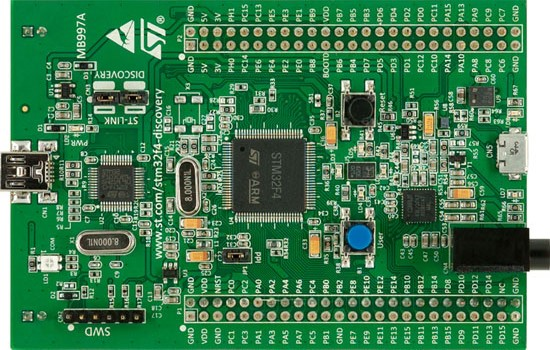
\includegraphics[width=0.6\textwidth]{bilder/stm32.jpg}
  \caption{STM32F4 Discovery board, USB port for debugging and programming on the left, USB port connected to the
    STM32F407 on the right.}
  \label{fig:stm32}
\end{figure}

The whole device consists of a single PCB onto which the STM32F4 Discovery board is mounted. This board has connections
for the impedances to be measured, a power supply jack, as well as a header where calibration resistors are mounted.
A picture of the front and back side of the finished board can be seen in \autoref{fig:pcb_frontback}
(\autopageref{fig:pcb_frontback}). Aside from the fitted components described later, there are footprints and traces
for a USB host connector (to save measurements onto a USB flash drive), an Ethernet jack (for remote control over
an IP network) and two additional memory chips. These features are not yet implemented in the firmware.

\begin{figure}[htpb]
  \centering
    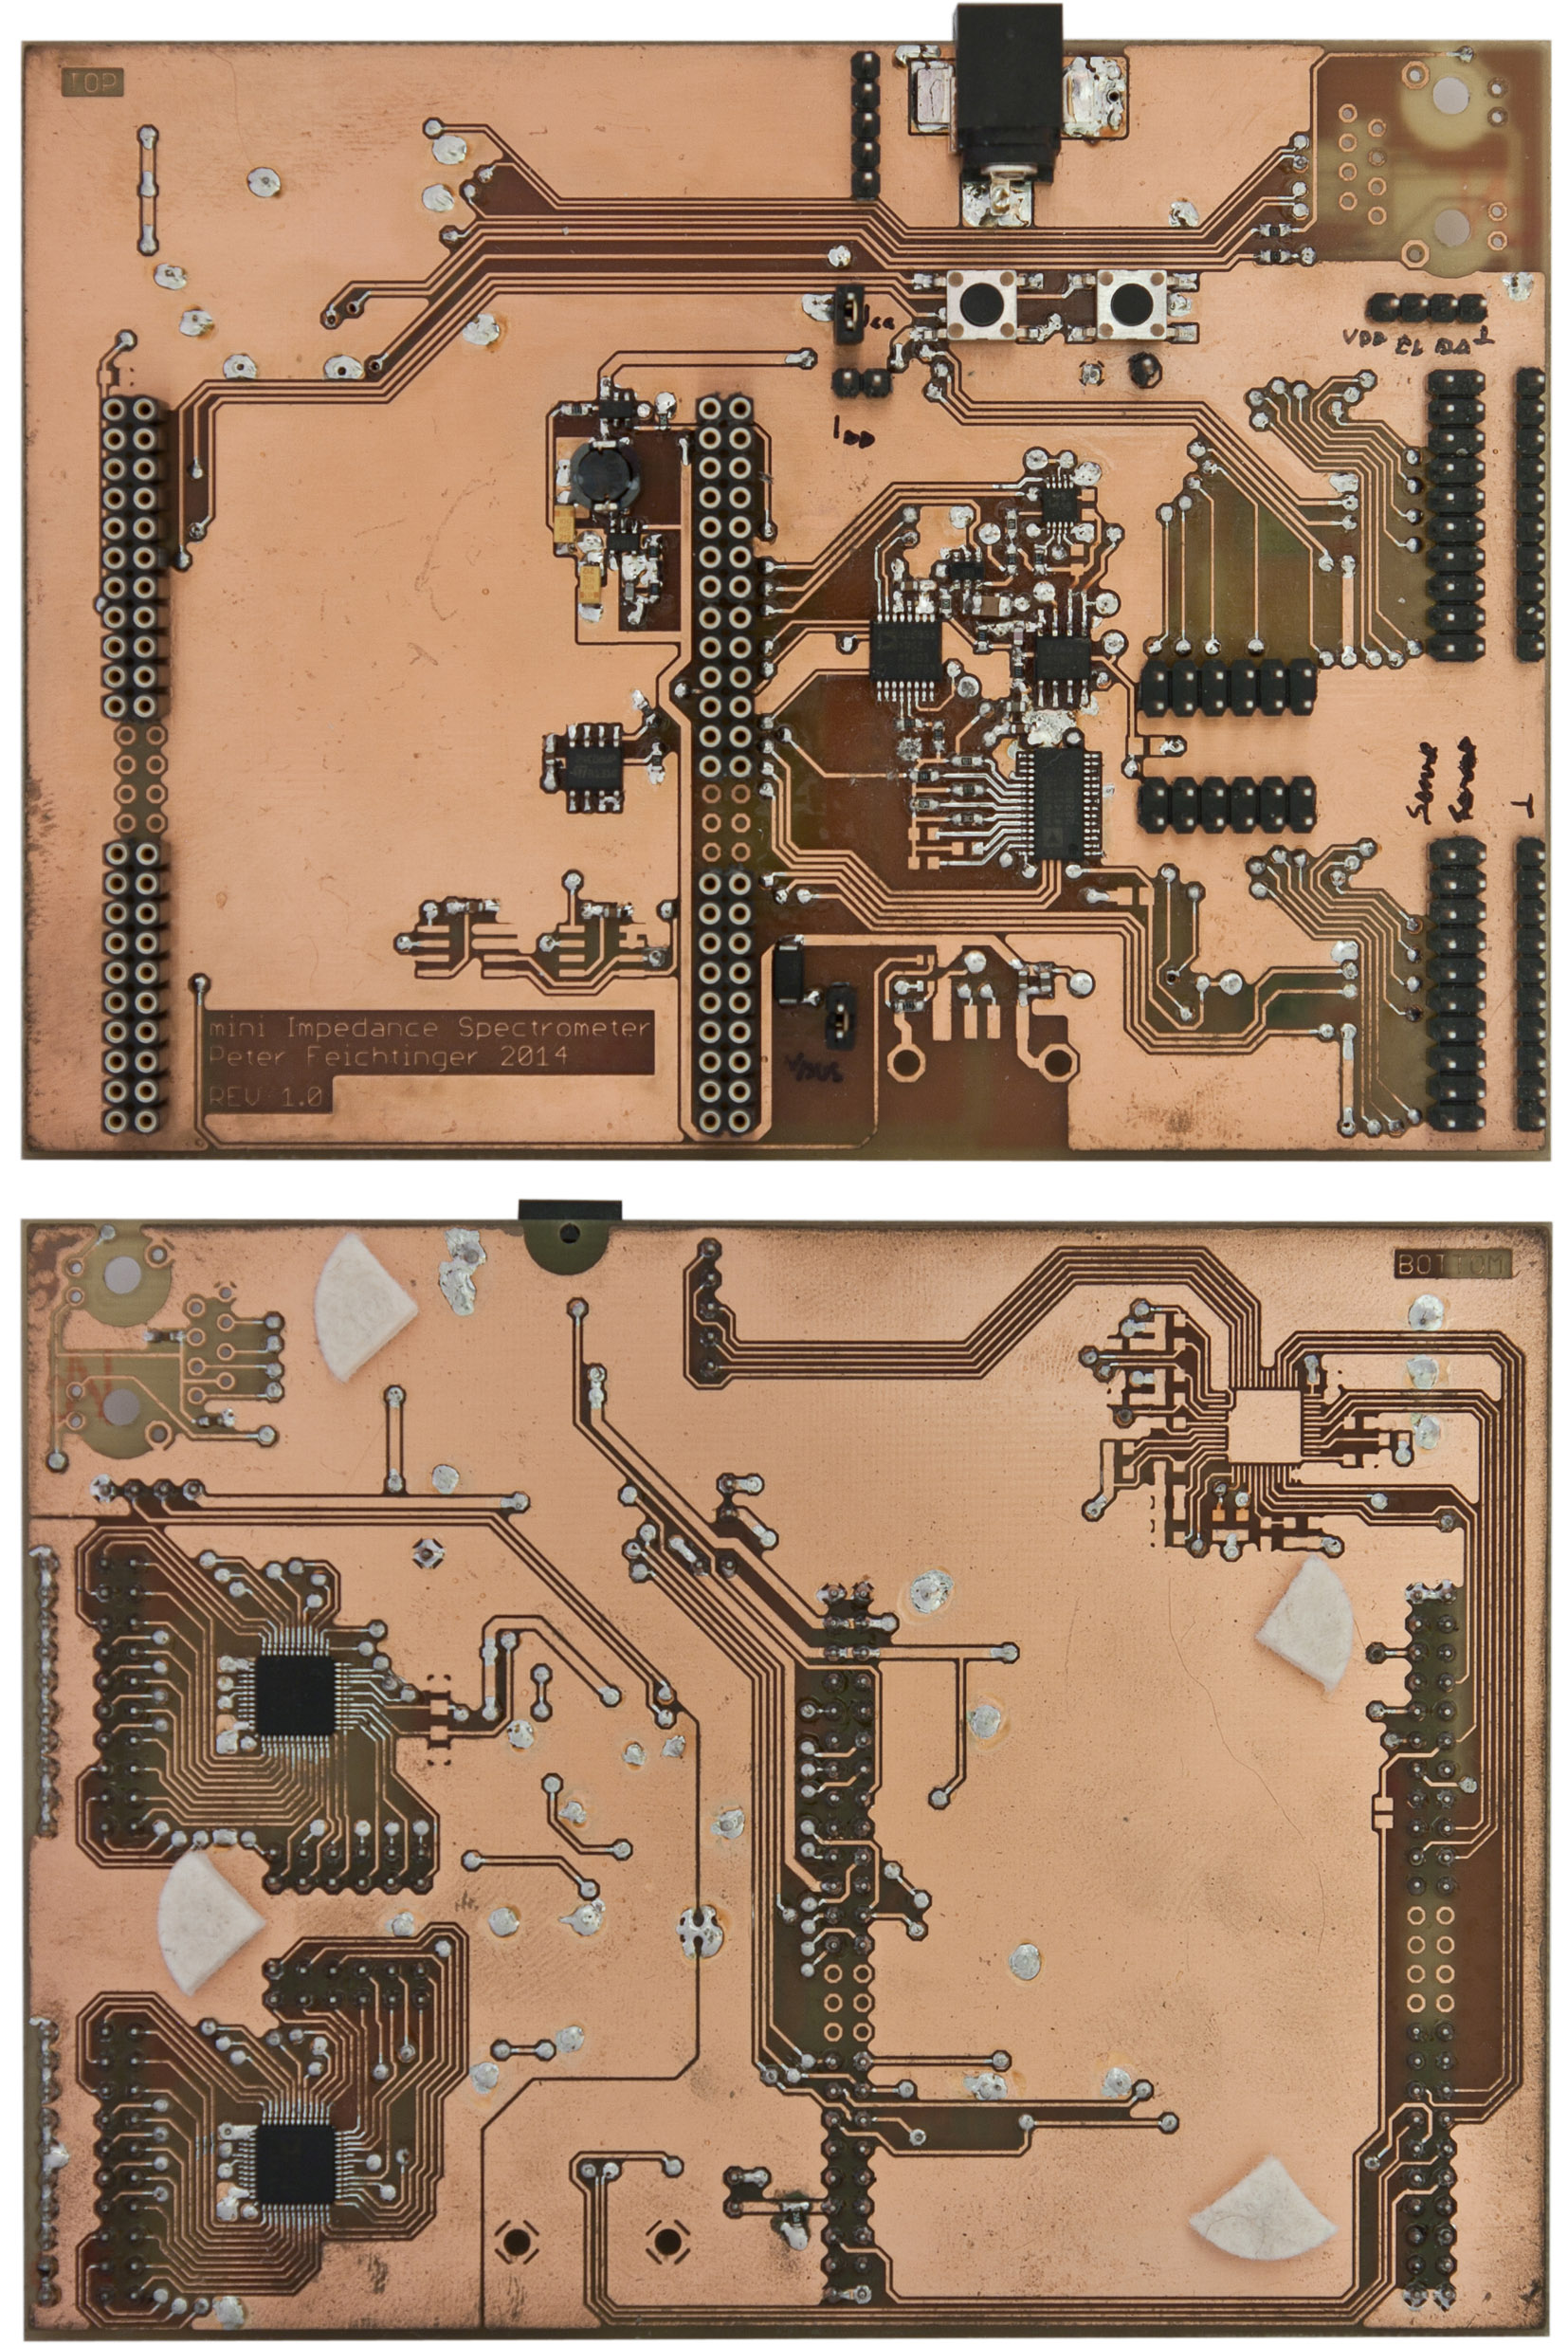
\includegraphics[width=\textwidth]{bilder/pcb_frontback.jpg}
  \caption{Front and back side of the populated PCB, the STM32F4 Discovery board is mounted on the left, unknown
    impedances are connected on the right. A board with calibration resistors can be connected left of the measurement
    connectors.}
  \label{fig:pcb_frontback}
\end{figure}

The complete schematics for the board can be found in \autoref{sec:schematics}.


\section{The AD5933}

This section will describe the AD5933 and the impedance measurement procedure in particular, providing information
from the datasheet\footnotemark{} in a digested form.
A block diagram of the AD5933 can be seen in \autoref{fig:ad_block} (\autopageref{fig:ad_block}).
\footnotetext{Analog Devices, \enquote{1 MSPS, 12-Bit Impedance Converter, Network Analyzer,} AD5933 datasheet,
  May 2013 [Rev.\ E]: \url{http://www.analog.com/static/imported-files/data_sheets/AD5933.pdf}}

\begin{figure}[htpb]
  \centering
    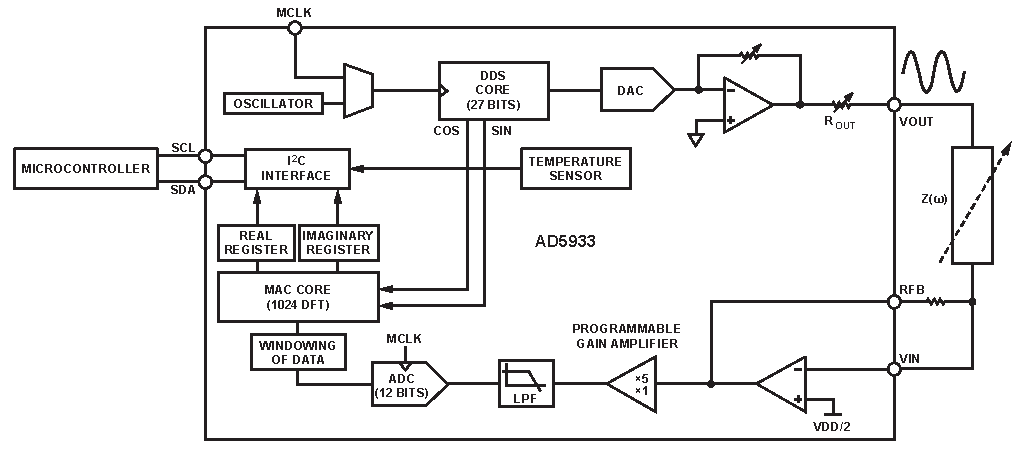
\includegraphics[width=\textwidth]{bilder/ad_block.pdf}
  \caption{Block diagram of the AD5933 showing the digital and analog parts, connected to a micrcontroller
    and an impedance that is measured, respectively.}
  \label{fig:ad_block}
\end{figure}


\subsection{Measurement Procedure} \label{sec:ad5933_proc}

To measure an unknown impedance, it is excited with a known voltage at a known frequency, both of which are programmed
via the \iic{} interface.

The AD5933 DDS core generates a sine wave at a desired frequency, which is converted to analog and output by the
internal output amplifier. The output amplifier can be configured by software to different voltage levels
(approximately \unit{200}{\milli\volt}, \unit{380}{\milli\volt}, \unit{1}{\volt} or \unit{2}{\volt} peak-to-peak with
a \unit{3.3}{\volt} supply), each having a different DC offset voltage and amplifier output resistance.
The unknown impedance is connected between the output amplifier and the input amplifier. The input amplifier works as
a current-to-voltage converter and needs an external feedback resistor, which is used to set the converter ratio
and therefore influences the possible range of the unknown impedance.
The input voltage (which is proportional to the current flowing through the measured impedance) is converted to digital
after low-pass filtering and windowed for the FFT computation.
The DSP engine then calculates a Fourier transform of the input signal in relation to the output signal,
which results in the raw real and imaginary impedance values that can be read from the AD5933 registers.

Since the phase shift introduced by the system and the overall gain of the amplifiers are unknown, these values can't
be used directly, but a calibration measurement with a known resistor needs to be made. A resistor is used because
it doesn't introduce a phase shift of its own.
From the calibration measurement data $ Z_\text{RAW} $, gain factor and system phase are calculated by
\begin{align}
  GF &= \left| Z_\text{RAW} \right| \cdot Z_\text{CAL} , \\
  \varphi_\text{SYS} &= \angle\, Z_\text{RAW}.
\end{align}
For an unknown impedance, the actual magnitude and phase are then calculated by
\begin{align}
  \left| Z \right| &= \frac{GF}{\left| Z_\text{RAW} \right|} , \\
  \angle\, Z &= \angle\, Z_\text{RAW} - \varphi_\text{SYS}.
\end{align}

On the controlling side of things, the AD5933 is programmed with a starting frequency, a frequency increment, the
number of increments in a sweep and the number of settling cycles.
A sweep is then started by writing two commands to the control register, \emph{initialize with start frequency} and
\emph{start frequency sweep}. Unfortunately, the AD5933 has no interrupt capability, so the status register needs to
be queried periodically, to determine when a frequency point has been measured. The raw values are then read and an
\emph{increment frequency} or \emph{repeat frequency} command is programmed. When all points have been measured
(that is, the frequency has been incremented the set number of times), a bit in the status register is set to signal a
complete sweep.
The number of settling cycles mentioned earlier determines, how long the AD5933 waits between a change
in the output frequency and the start of the analog-to-digital conversion, giving the measured impedance time to
settle to the new frequency.

Because of the limited number of 1024 sampling points used when calculating the Fourier transform,
the frequency range with any one clock frequency is limited. Using the internal oscillator with
\unit{16.667}{\mega\hertz}, the ADC samples with \unit{1}{\mega{}S\per\second}, which limits the upper frequency to
about \unit{100}{\kilo\hertz} (above which the phase error increases significantly) and the lower frequency to about
\unit{10}{\kilo\hertz} to \unit{1}{\kilo\hertz} (depending on the desired accuracy).
To measure lower frequencies, an external clock source has to be used, which is supplied by an STM32F407 timer output.


\subsection{Analog Front End (AFE)}

The AD5933 has some severe limitations concerning its output and the load that can be placed there. Without additional
circuitry, the range is limited to at least a few \unit{100}{\kilo\ohm} up to \unit{10}{\mega\ohm}.
This limitation is caused by the significant output resistance of the output amplifier, which can be as high as
\unit{2.4}{\kilo\ohm}, as well as the output offset voltage, which limits the dynamic range of the input amplifier.

Since the desired range is down to about \unit{10}{\ohm}, and more than one impedance should be measured at once,
an external analog front end is used.
A block diagram of the external AFE can be seen in \autoref{fig:afe_block}.
There are four analog multiplexers (dual ADG725 by Analog Devices, M1 in the schematic) that connect multiple unknown
and calibration impedances in a four-wire arrangement, to cancel out the on-resistance of the multiplexers.
Multiplexer M2 is used to attenuate the output voltage of the AD5933, this is needed when measuring small impedances,
so the output current is kept small.
Multiplexer M3 switches between different feedback resistors to change the I-U conversion ratio.

\begin{figure}[hpb]
  \centering
    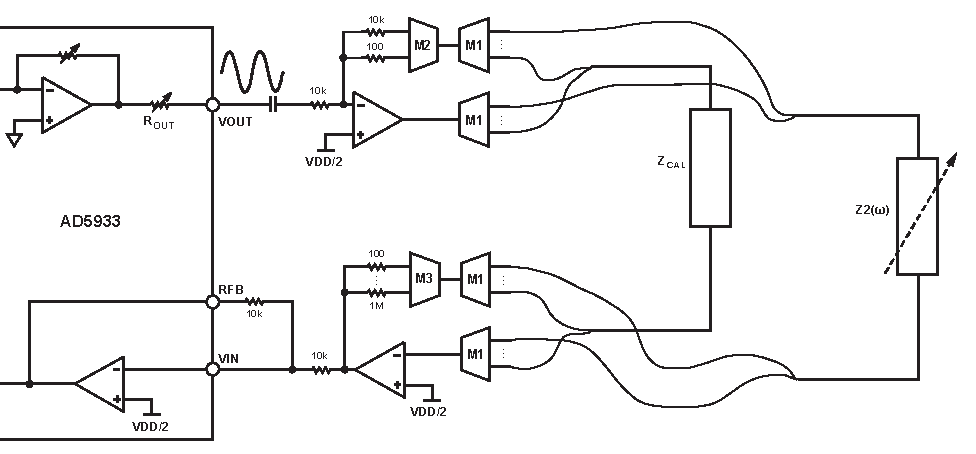
\includegraphics[width=\textwidth]{bilder/afe_block.pdf}
  \caption{Block diagram of the AD5933 output stage with external analog front end and calibration impedance.}
  \label{fig:afe_block}
\end{figure}

The two op-amps are AD8656 by Analog Devices, the one in the output stage is configured as an inverting amplifier,
the one on the input as a current-to-voltage converter, with the AD5933-internal input amplifier acting as an inverting
voltage follower. The coupling capacitor between AD5933 output and the output amplifier filters the DC offset so the
whole input voltage range can be used.

In this configuration, the impedance range is limited by the maximum output current of the
op-amps and their closed-loop output impedance, which either needs to be small enough so it can be ignored compared
to the unknown impedance, or characterized over the whole frequency range so it can be taken into account properly.


\section{Power Supply and Memory}

Although the STM32F4 Discovery board already has a \unit{3.3}{\volt} voltage regulator that could be used, a
switching regulator (LTC3406 by Linear Technology) is included on the board. This has mainly two reasons:
\begin{itemize}
	\item for the excitation voltage of the unknown impedance to be well known, the power supply needs to be
    reasonably accurate and
  \item it should be possible to power the device from a standard USB 2.0 port, which can supply a maximum current of
    \unit{500}{\milli\ampere}. Considering that a USB host port can be added, which should in turn be able to power
    a standard USB flash drive, power conversion efficiency needs to be as high as possible. 
\end{itemize}

Since the STM32F407 doesn't have any non-volatile memory, an EEPROM is added to store some static configuration
options (e.g.\ fitted feedback resistors, possible output voltage attenuations or the Ethernet MAC address) as well as
dynamic settings such as the frequency range and output voltage used last. Like the AD5933, this memory is connected
via \iic{} to the microcontroller.


\section{Unpopulated Peripherals}

During the hardware design, some interesting peripherals were included in the board schematic, as well as the PCB
layout. Since programming the firmware to use these would have been beyond the scope of this thesis, they are not
populated on the final board.

These peripherals include
\begin{itemize}
  \item external SRAM and flash memory,
	\item an Ethernet jack and PHY,
  \item a USB host plug.
\end{itemize}
To populate and use them, only the respective modules need to be added to the firmware, aside from the necessary
changes, should the PCB layout be bad.
